\item A $3 \times 3$ image $\vec{A}$ has been linearly stretched to get the maximum contrast in an $8$-bit display system. Digital Number (DN) values of the pixels in image $\vec{A}$ are shown. The value of the pixel marked as `?' in the output image $\vec{B}$ after linear stretching is \rule{1cm}{0.01pt}. 
\hfill{\brak{\text{GG 2025}}}
\begin{figure}[H]
    \centering
    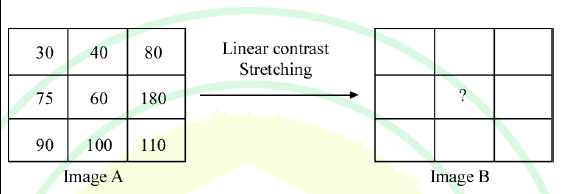
\includegraphics[width=0.7\columnwidth]{GATE/2025/GG1/figs/fig12.png}
    \caption{}
    \label{fig:q63}
\end{figure}

